\documentclass[twocolumn]{article}
\usepackage{graphicx}
\usepackage{amsmath}
\usepackage{hyperref}

\begin{document}
\title{Final Exam: Inverse iteration algorithm for eigenvalues}
\author{Simon Vendelbo Bylling Jensen\thanks{AU E-mail: 201507956@uni.au.dk} \thanks{CERN E-mail: simon.vendelbo.jensen@cern.ch}\\
Stud. Nr. 201507956 \\
Au Id. Au545766}
\date{\today}
\maketitle

\begin{abstract}
The  solution of exercise 10 for the final exam. An implementation of an inverse iteration algorithm for eigenvalues and eigenvectors. Such an implementation has been made, the first relying on a Golub-Kahan-Lanczos bidiagonalization, thereby also solving exam exercise 9, and   iterating using a calculated matrix-inverse, as well as a method using QR-decomposition by modified Gram-Schmidt orthogonalization to iterate through the solution of a linear system using backsubstitution.
\end{abstract}

\section*{Introduction and Problem}
I have received exercise number 10, since my student number 56, which by modulus 23 will give 10. The problem is to implement a variant of the inverse iteration method that calculates the eigenvalue closest to a given number $s$ and returns the corresponding eigenvector. The problem of finding eigenvalues and corresponding eigenvectors are crucial to various fields of physics and engineering. Especially for highly complicated quantum systems, complicated engineering systems and much more, the task of finding an individual eigenvalue and determine its corresponding eigenvectors is essential. The algorithm, which will be demonstrated is a fast and effective way of doing exactly that.

At first the implementation and theory of the inverse iteration method will be described in Sec. \ref{sec:0} and afterwards the different related methods will be compared and analysed in Sec. \ref{sec:5}. Implementations and simple calculations using the examined methods will similarly be demonstrated in the main.c file, and which results can be found in the out.txt file, as well as described hereafter.

\section{\label{sec:0}Implementation and Theory}
The implementation and theory all relies on the lecture notes from Ref. \cite[Chapter 12 - Eigenvalues 2: Power methods and Krylov subspace methods]{Dmi}. The refined inverse iteration method relies on a few simple principles. All of these principles will be described by different examples, which are all demonstrated in the main.c file, and which results can be found in the out.txt file. The description of the inverse iteration method will thereby be formulated by first examining simpler implementations of the same procedure. This will be the case for Secs. \ref{sec:1} to \ref{sec:4}.

\subsection{\label{sec:1}The Power Method}
Since the inverse iteration method is a cleverly designed power method, it is essential to introduce the basics of the power methods. The simplest power method is the power iteration, which works by multiplying a random vector $\vec{V}$ on a matrix $A$ of similar size, where we want to know the largest eigenvalue and corresponding eigenvector of $A$. By continuously multiplying the vector $\vec{V}$ on the matrix $A$, through the iteration
\begin{equation}
\vec{V}_{i+1} = A \vec{V}_i \label{eq:1}
\end{equation}
we are able to approximate the largest eigenvector and largest eigenvalue very cleverly. The vector will at some point simply converge to the largest eigenvector.  This is since by the multiplication, the dimension in which the eigenvector corresponding to the numerically largest eigenvalue will give the largest enhancement of the vector, $\vec{V}$, and for each iteration, this will have positive feedback and will at some point have $\vec{V}$ converge to some vector, which normalized will approximate exactly the largest eigenvector. The algortim in the functionfile.c are constructed with an automatic renormalization feature, such that the algorithm will not give errors do to the lach of accurary of the large numbers, which will be multiplied. 
 If the vector $\vec{V}$ will converge to the eigenvector, then at some point every iteration will fulfill the eigenvector identity
\begin{equation}
A \vec{V}_\lambda = \lambda \vec{V}_\lambda. \label{eq:2}
\end{equation}
We will thereby be able to approximate the largest eigenvalue continuously by finding the factor, in which $\vec{V}$ increases for every iteration. This parameter are continuously detected and are called the Rayleigh quotient. This will due to Eq. \eqref{eq:2} at some point converge to the largest eigenvalue. This Rayleigh quotient is given as
\begin{equation}
\lambda \left[ \vec{V}_i \right] = \frac{\vec{V}^T_i A \vec{V}}{\vec{V}_i \cdot \vec{V}_i}. \label{eq:3}
\end{equation}
For the implementation in the main.c file the satisfaction criteria for when an eigenvalue has been found, is when this Rayleigh quotient have converged and do not change with an iteration. This power method is particularly effective in use, since it do not have to do any large matrix decompositions, which the computation of eigenvalues usually requires.

\subsection{\label{sec:2}The Inverse Power Method}
Intuitively when one would be able to converge to the numerical largest eigenvalue by continuously multiplying with the matrix $A$ one would expect, that a similar procedure could be done to find the numerically smallest eigenvalue. This is true, but the cost of this implementation, is the fact that one would in this case have to calculate the inverse of the matrix $A$. By the similar argument as for the power method, by multiplying with the inverse of $A$, the minimum eigenvalue will now be dominant and the vector $\vec{V}$ will converge to the corresponding eigenvector. The iterations are hereby similar to Eq. \eqref{eq:1} and given as
\begin{equation}
\vec{V}_{i+1} = A^{-1} \vec{V}_i. \label{eq:4}
\end{equation}
The inverse are for this case found using the Golub-Kahan-Lanczos bidiagonalization as previously implemented in the Linear Equation exercise C and which is the final exam question 9. This procedure is described in the following subsection \ref{sec:2.2}. When the inverse is found, one can continuously apply iteration in Eq. \eqref{eq:4} to find the most dominant eigenvector when inverse iterating. This will be the eigenvector with the numerical smallest eigenvalue. To avoid reaching machine epsilon doing this procedure, a renormalization has been implemented, which do not effect the efficiency of the code significantly. 
This time since we apply the $A^{-1}$ instead of $A$, the eigenvector identity now becomes
\begin{equation}
 A^{-1} \vec{V}_\lambda = \frac{1}{\lambda} \vec{V}_\lambda, \label{eq:5}
\end{equation}
instead of Eq. \eqref{eq:2}. And therefore the Rayleigh parameter from Eq. \eqref{eq:3} will not be approximating the lowest numerical eigenvalue, but instead it will  be approximating the inverse of the lowest numerical eigenvalue.
 
\subsubsection{\label{sec:2.2}Golub Kahan Lanczos Bidiagonalization}
The Goloub Kahan Lanczos bidiagonalization is the subject of the final exam exercise 9, and the linear-equation exercise C. It provides an efficient way of finding the inverse of a function, which is needed in the inverse power method. The procedure of implementing this is described in Ref. \cite{GKL}. The method is usually the start of a single value decomposition, and work by computing the unitary orthogonal matrices $U$ and $V$, such that
\begin{equation}
U^\ast A V = B,
\end{equation}
where $B$ is bidiagonal. This procedure is related the Gram-Schmidt orthogonalization procedure, since it starts with a vector from both $V$ and $U$, then it orthogonalize it to the previous vectors and it normalizes the vector. However opposed to the simple Gram-Schmidt procedure, the Golub Kahan Lanczos bidiagonalization makes sure, through relations
\begin{align}
\alpha_k \vec{U}_{k} &= A\vec{V}_k - \beta_{k-1} \vec{U}_{k-1}, \\
\beta_k \vec{V}_{k+1} &= A^{\ast}\vec{U}_k - \alpha_k \vec{V}_k,
\end{align}
with $\alpha_k = \vec{U}_k^\ast A \vec{V}_k$ and $\beta_k = \vec{U}_k^\ast A \vec{V}_{k+1}$ to be able to provide a quicker inverse of a matrix. This is since the Gram-Schmidt procedure will return a triangular matrix, which can be used for finding the inverse through backpropagation. Here the Golub Kahan Lanczos method returns a matrix $B$, that will be quicker to solve through backpropagation, since it is bidiagonal opposed to triangular. The solution for the inverse, can thereby easily be found, by backsubstitution of the linear system
\begin{align}
A \cdot A^{-1} &= I,\\
U B V^T A^{-1} &= I,\\
B \left(V^T  A^{-1}\right) &= U^T.
\end{align}
This linear system is then solved for $V^T  A^{-1}$ which can be multiplied with the orthogonal $V$ to find the inverse. Many other aspects of this algorithm could be widely covered, but since this is not the point of the exercise, we will settle with the fact that the Golub Kahan Lanczos bidiagonalization procedure are able to provide us with $A^{-1}$ for the inverse power method.

\subsection{\label{sec:3} Shifted Inverse Iteration}
Since we in the final iteration method want to estimate an eigenvalue with corresponding eigenvector, which is close to a given value $s$ and is not necessarily the largest or the smallest eigenvalue, we need to implement a new method. The method will have to converge to a given region of eigenvalues. This is done using the previous inverse iteration method, since it converges to a controlled value $0$, which then has to be shifted to the given point $s$.
This can be very simply executed with an understanding of the linear algebra of eigenvalues and eigenvectors. If one apply the shift
\begin{equation}
A \rightarrow A - sI, \label{eq:shift}
\end{equation}
any eigenvectors of $A$ will on this shifted matrix still remain an eigenvector, and through Eq. \eqref{eq:2} give
\begin{align}
\left(A - s I\right) \vec{V}_\lambda &=  A \vec{V}_\lambda - s I \vec{V}_\lambda, \\
 &= \lambda \vec{V}_\lambda  -  s \vec{V}_\lambda, \\
 &= \left(\lambda - s\right) \vec{V}_\lambda.
\end{align}
Thereby introducing a shifted eigenvalue by Eq. \eqref{eq:shift}, one can simply use the inverse power method with iterations as
\begin{equation}
\vec{V}_{i+1} = \left(A - sI\right)^{-1} \vec{V}_i \label{eq:6}
\end{equation}
to find any eigenvalues, with the expected eigenvalue area around $s$. Since these eigenvalues now will be shifted to be close to $0$ where the previous inverse power method will converge to them. Afterwards one must remember to shift eigenvalue back by the same $s$, to find its actual location, whereas the eigenvector remains the same. This procedure has been implemented and tested in the main.c file using Golub Kahan Lanczos bidiagonalization method to find the inverse of the shifted $\left( A - sI \right)$.
A more refined way of doing the shifted inverse power method is the inverse iteration method, in which one do not need to calculate the inverse of $A$, but instead solves a linear system. This will now follow.

\subsection{\label{sec:4} Inverse Iteration Method}
The main difference in the inverse power method and this refined inverse iteration method is the change from iteration through multiplication as in Eq. \eqref{eq:6}, to now iterate through finding the next vector by solving the linear system
\begin{equation}
\left(A - sI\right) \vec{V}_{i+1} =  \vec{V}_i \label{eq:7}
\end{equation}
This could in fact be done by the previously defined Golub-Kahan-Lanczos bidiagonalization method, since this will end up in a backsubstitution, which is significantly simpler for the bidiagonalized matrices. However we need to consider another procedure of solving these systems, namely the QR-decomposition by modified Gram-Schmidt orthogonalization. Such an implementation has been made as in the linear equation exercise B. This method will be discussed in the following subsection, but differs from the Golub Kahan Lanczos bidiagonalization method by being faster to compute initially, since it only needs to construct a single orthogonal matrix. But since the triangular matrix from the QR decomposition is slower to make a complete backsubstitution of, than the quick backsubstitution of the bidiagonalized matrix, then the main difference between these two methods for this implementation is the QR-decomposition being quicker to initialize, but more costly per iteration, whereas the Golub-Kahan-Lanczos method is more costly to initialize, but quicker to run. Since we want to implement an algorithm, that allows the user to specify how often the system should replace the user provided $s$ with the estimated eigenvalue from the Rayleigh quotient, whereas the QR or Golub-Kahan-Lanczos method would be reinitialized, then for a demonstration of an inverse iteration algorithm with many continuous updates, the QR-decomposition will be the fastest, and for one in which the user-supplied estimate is very accurate, and one would not need to replace it with any estimate from the Rayleigh quotient, one would prefer the Golub-Kahan-Lanczos method, especially if a lot of iterations are needed. \\

In Ref. \cite[Chapter 12 - Eigenvalues 2: Power methods and Krylov subspace methods]{Dmi} it states that in practise the method is usually used for finding a result when a good approximation for the eigenvalue is known, with only a few iterations. If only a few iterations shall be made, then the fast initialized QR-decomposition should be the fastest, and therefore the one we will choose for the iteration procedure.

The QR-decomposition will be described in the following Sec. \ref{sec:4.2}, and will through backsubstitution determine the new step at each iteration. Again to avoid reaching machine epsilon doing this procedure, a renormalization has been implemented, which do not effect the efficiency of the code significantly. With the optimized iteration step, the rest of the inverse iteration method is simply implemented as for the shifted inverse power method as described in Sec. \ref{sec:2}.

\subsubsection{\label{sec:4.2}QR-Decomposition by modified Gram-Schmidt orthogonalization}
The QR-decomposition in use for solving the linear system from Eq. \eqref{eq:7} is very simple, and previously examined in the linear equation exercise A. The key of this method is expressing a matrix $A$ as a product of a orthogonal matrix $Q$ and a right triangular matrix $R$ as
\begin{equation}
A = QR.
\end{equation}
From being orthogonal, we know that $Q$ satisfies $Q^T Q = 1$ and this way we can by multiplying with $Q^T$ from the left of any linear system find
\begin{align}
A \vec{x} &= \vec{b}\\
QR \vec{x} &= \vec{b}\\
R \vec{x} &= Q^T \vec{b}
\end{align}
Where since $R$ is a right triangular matrix, we simply need to solve this by a backsubstitution. This way, a solution to any linear problem can be solved through QR-decomposition, a multiplication of $Q^T$ and a backsubstitution. The QR-decomposition can be done in multiple ways, but the one in use is the method of orthogonalization through the Gram-Schmidt process. This process takes the set of vectors $\vec{a_i}$ which $A$ consists of, and generates an orthogonal set $\vec{q_i}$, which spans the same subspace as $A$. This is done one vector at the time, and the process consists of removing the compartment of any of the vectors $\vec{a_j}$ that is spanned by the made vector of the new orthogonal set $\vec{q_i}$ to ensure orthogonality. This is done after normalization through the typical inner product by the procedure
\begin{align}
\vec{q_i} &= \frac{\vec{a_i}}{\mid \mid \vec{a_i} \mid \mid} ,\label{eq:norm}\\
\vec{a_i'} &= \vec{a_i} - \sum_{i \neq j} \langle \vec{q_i} \mid \vec{a_i} \rangle \vec{q_i}. \label{eq:project}
\end{align}
Since this procedure always makes sure that any new vector $\vec{q_i}$ is orthonormal and orthogonal to even all of the states $\vec{a_i}$, which are continuously modified with the calculation of a new $\vec{q_i}$, this method is referred to as the stabilized or modified Gram-Schmidt procedure. Using this procedure we are able to find the matrix $Q$ consisting of the vectors $\vec{q_i}$ which span the same subspace as $A$. However in order to complete this QR-decomposition we still need to consider the $R$-matrix. This represents the mapping to be done if the orthonormal basis $Q$ are to be mapped onto the matrix $A$. Therefore this matrix must consist of the inverse of all the the projections and normalisations as done to construct $Q$ from $A$. Therefore the diagonal of $R$ consists of the norm removed when normalizing for retrieving $Q$ through Eq. \eqref{eq:norm} by
\begin{equation}
R_{ii}= \mid \mid \vec{a_i} \mid \mid,
\end{equation}
and the upper triangular elements consist of the projections, which were previously removed in Eq. \eqref{eq:project},
\begin{equation}
R_{ij}= \vec{q_i}^T \vec{a_j}.
\end{equation}
Since we are dealing with the stabilized procedure we must modify the vectors $\vec{a_j}$ to include the projection elements as
\begin{equation}
\vec{a_j'} = \vec{a_j}  - \vec{q_i} R_{ij}.
\end{equation}
Using these equations one can QR-decompose the linear system of Eq. \eqref{eq:7}, to find the next iteration in the inverse iteration method. This procedure concludes the theory and implementation section.

\section{\label{sec:5}Comparison and Results}
An implementation of firstly the inverse iteration method, but also all other methods have been made and are tested in the main.c file. If one wants to check the calculation through an individual test of these methods, this will be provided in the out.txt file for inspection. The inverse iteration method is made such that it takes five inputs. These five are the matrix in which we want to find the eigenvalues, an empty vector for the function to output the found eigenvalue, an empty vector for the function to return the eigenvector corresponding to the eigenvalue, an estimate of the eigenvalue from which the method will search, and the number of iterations that the user would prefer the program to take, before it re-estimates the eigenvalue for improving the subsequent iterations.

In order to conclude anything based on the implemented refined inverse iteration method described in Sec. \ref{sec:4} as well as similar methods as described in Sec. \ref{sec:1} to \ref{sec:3}, a comparison must be made to each other. To furthermore make sure that any inconsistencies might not appear in all four methods, a comparison has also been made to the classic Jacobi eigenvalue algorithm from the exercise C on eigenvalues, which makes it possible to correct the found eigenvalues and eigenvectors. This procedure is all done in the main.c file and can be viewed in the out.txt file.


Furthermore since the Jacobi algorithm from exercise B on eigenvalues returns a single eigenvalue just as the inverse iteration method, it will make a good benchmark for the speed of the inverse iteration method.  Since these Jacobi methods only works as a benchmark and are not a part of the implementation of the inverse iteration method, the theory behind these will not be discussed here, but it is described in the Ref. \cite[Chapter 3 - Eigenvalues and eigenvectors]{Dmi}.

In the following Sec. \ref{sec:6}, firstly a comparison between the models discussed in Sec. \ref{sec:1} to \ref{sec:4} will be made and the results will be discussed. Hereafter a in depth analysis of the opportunity to re-update the estimate of the eigenvalue at certain steps of the method will be made and compared to test results in Sec. \ref{sec:7}. At last the inverse iteration method will be compared to the Jacobi diagonalization method for finding only one eigenvalue at different matrix-sizes in Sec. \ref{sec:8}.

\subsection{\label{sec:6}Power Iteration Methods}
To compare the individual implemented power iteration algorithms for finding an eigenvalue, one must consider different aspects. These codes will all require more iterations if two targeted eigenvalues are almost equal in size. Therefore the power method of Sec. \ref{sec:1} is difficult to rightfully compare to the inverse power methods, however since it do not need to find any inverse matrices or solve any linear equations it can be expected to be a bit faster in most cases. The inverse power method of Sec. \ref{sec:2} and the shifted inverse power method of Sec. \ref{sec:3} should be identical if the shift is set to be $0$, these can therefore be compared in that region, where they should converge. If the shift is set to $0$ one could similarly compare the inverse iteration method of Sec. \ref{sec:4} to these two. This will not only compare the difference between the Golub-Kahan-Lanczos bidiagonalization compared to the QR-decomposition, but also compare the difference between computing the inverse of Eq. \eqref{eq:6} opposed to solving the linear system as in Eq. \eqref{eq:7}. This is of cause only a valid comparison if the refined inverse iteration algorithm is set to not continuously update its estimate of the eigenvalue for the improved iteration procedure. The effect of this degree of freedom will be discussed later in Sec. \ref{sec:7}. A test computing one eigenvalue on random matrices with dimension from $n=3$ to $n=50$ has been made and is shown in Fig. \ref{fig1}.

  \begin{figure}[h]
% GNUPLOT: LaTeX picture with Postscript
\begingroup
  \makeatletter
  \providecommand\color[2][]{%
    \GenericError{(gnuplot) \space\space\space\@spaces}{%
      Package color not loaded in conjunction with
      terminal option `colourtext'%
    }{See the gnuplot documentation for explanation.%
    }{Either use 'blacktext' in gnuplot or load the package
      color.sty in LaTeX.}%
    \renewcommand\color[2][]{}%
  }%
  \providecommand\includegraphics[2][]{%
    \GenericError{(gnuplot) \space\space\space\@spaces}{%
      Package graphicx or graphics not loaded%
    }{See the gnuplot documentation for explanation.%
    }{The gnuplot epslatex terminal needs graphicx.sty or graphics.sty.}%
    \renewcommand\includegraphics[2][]{}%
  }%
  \providecommand\rotatebox[2]{#2}%
  \@ifundefined{ifGPcolor}{%
    \newif\ifGPcolor
    \GPcolortrue
  }{}%
  \@ifundefined{ifGPblacktext}{%
    \newif\ifGPblacktext
    \GPblacktexttrue
  }{}%
  % define a \g@addto@macro without @ in the name:
  \let\gplgaddtomacro\g@addto@macro
  % define empty templates for all commands taking text:
  \gdef\gplbacktext{}%
  \gdef\gplfronttext{}%
  \makeatother
  \ifGPblacktext
    % no textcolor at all
    \def\colorrgb#1{}%
    \def\colorgray#1{}%
  \else
    % gray or color?
    \ifGPcolor
      \def\colorrgb#1{\color[rgb]{#1}}%
      \def\colorgray#1{\color[gray]{#1}}%
      \expandafter\def\csname LTw\endcsname{\color{white}}%
      \expandafter\def\csname LTb\endcsname{\color{black}}%
      \expandafter\def\csname LTa\endcsname{\color{black}}%
      \expandafter\def\csname LT0\endcsname{\color[rgb]{1,0,0}}%
      \expandafter\def\csname LT1\endcsname{\color[rgb]{0,1,0}}%
      \expandafter\def\csname LT2\endcsname{\color[rgb]{0,0,1}}%
      \expandafter\def\csname LT3\endcsname{\color[rgb]{1,0,1}}%
      \expandafter\def\csname LT4\endcsname{\color[rgb]{0,1,1}}%
      \expandafter\def\csname LT5\endcsname{\color[rgb]{1,1,0}}%
      \expandafter\def\csname LT6\endcsname{\color[rgb]{0,0,0}}%
      \expandafter\def\csname LT7\endcsname{\color[rgb]{1,0.3,0}}%
      \expandafter\def\csname LT8\endcsname{\color[rgb]{0.5,0.5,0.5}}%
    \else
      % gray
      \def\colorrgb#1{\color{black}}%
      \def\colorgray#1{\color[gray]{#1}}%
      \expandafter\def\csname LTw\endcsname{\color{white}}%
      \expandafter\def\csname LTb\endcsname{\color{black}}%
      \expandafter\def\csname LTa\endcsname{\color{black}}%
      \expandafter\def\csname LT0\endcsname{\color{black}}%
      \expandafter\def\csname LT1\endcsname{\color{black}}%
      \expandafter\def\csname LT2\endcsname{\color{black}}%
      \expandafter\def\csname LT3\endcsname{\color{black}}%
      \expandafter\def\csname LT4\endcsname{\color{black}}%
      \expandafter\def\csname LT5\endcsname{\color{black}}%
      \expandafter\def\csname LT6\endcsname{\color{black}}%
      \expandafter\def\csname LT7\endcsname{\color{black}}%
      \expandafter\def\csname LT8\endcsname{\color{black}}%
    \fi
  \fi
    \setlength{\unitlength}{0.0500bp}%
    \ifx\gptboxheight\undefined%
      \newlength{\gptboxheight}%
      \newlength{\gptboxwidth}%
      \newsavebox{\gptboxtext}%
    \fi%
    \setlength{\fboxrule}{0.5pt}%
    \setlength{\fboxsep}{1pt}%
\begin{picture}(4320.00,3456.00)%
    \gplgaddtomacro\gplbacktext{%
      \csname LTb\endcsname%%
      \put(645,669){\makebox(0,0)[r]{\strut{}$0$}}%
      \csname LTb\endcsname%%
      \put(645,994){\makebox(0,0)[r]{\strut{}$100$}}%
      \csname LTb\endcsname%%
      \put(645,1319){\makebox(0,0)[r]{\strut{}$200$}}%
      \csname LTb\endcsname%%
      \put(645,1644){\makebox(0,0)[r]{\strut{}$300$}}%
      \csname LTb\endcsname%%
      \put(645,1969){\makebox(0,0)[r]{\strut{}$400$}}%
      \csname LTb\endcsname%%
      \put(645,2294){\makebox(0,0)[r]{\strut{}$500$}}%
      \csname LTb\endcsname%%
      \put(645,2619){\makebox(0,0)[r]{\strut{}$600$}}%
      \csname LTb\endcsname%%
      \put(645,2944){\makebox(0,0)[r]{\strut{}$700$}}%
      \csname LTb\endcsname%%
      \put(645,3269){\makebox(0,0)[r]{\strut{}$800$}}%
      \csname LTb\endcsname%%
      \put(821,409){\makebox(0,0){\strut{}$0$}}%
      \csname LTb\endcsname%%
      \put(1341,409){\makebox(0,0){\strut{}$5$}}%
      \csname LTb\endcsname%%
      \put(1860,409){\makebox(0,0){\strut{}$10$}}%
      \csname LTb\endcsname%%
      \put(2380,409){\makebox(0,0){\strut{}$15$}}%
      \csname LTb\endcsname%%
      \put(2900,409){\makebox(0,0){\strut{}$20$}}%
      \csname LTb\endcsname%%
      \put(3419,409){\makebox(0,0){\strut{}$25$}}%
      \csname LTb\endcsname%%
      \put(3939,409){\makebox(0,0){\strut{}$30$}}%
    }%
    \gplgaddtomacro\gplfronttext{%
      \csname LTb\endcsname%%
      \put(153,1969){\rotatebox{-270}{\makebox(0,0){\strut{}Number of Iterations}}}%
      \csname LTb\endcsname%%
      \put(2380,130){\makebox(0,0){\strut{}Matrix Dimension "n"}}%
      \csname LTb\endcsname%%
      \put(3065,3102){\makebox(0,0)[r]{\strut{}Power Iter.}}%
      \csname LTb\endcsname%%
      \put(3065,2916){\makebox(0,0)[r]{\strut{}Inverse Power Iter.}}%
      \csname LTb\endcsname%%
      \put(3065,2730){\makebox(0,0)[r]{\strut{}Shifted Inverse Iter.}}%
      \csname LTb\endcsname%%
      \put(3065,2544){\makebox(0,0)[r]{\strut{}Inverse Iter.}}%
    }%
    \gplbacktext
    \put(0,0){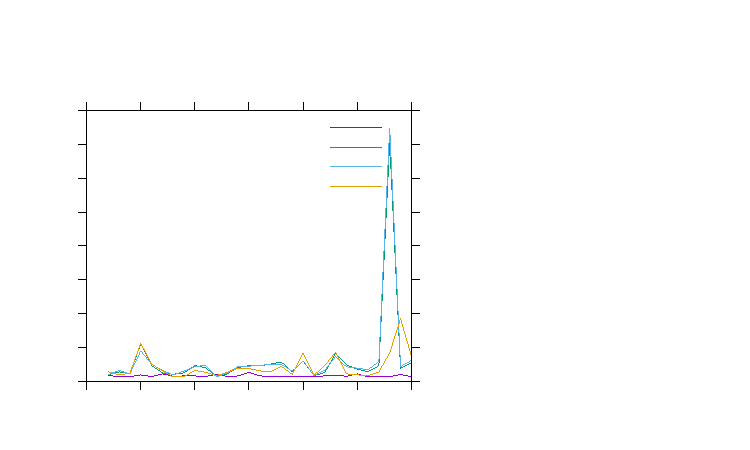
\includegraphics{plot-cairo}}%
    \gplfronttext
  \end{picture}%
\endgroup

\caption{Comparison between the number of iterations made by different power methods when estimating one eigenvalue of a random real symmetric matrix (values from $0$ to $10$), of different size $n$. The shift of the shifted inverse and inverse iteration method is set to $0$ and the inverse iteration method is set to not continuously update its estimate of the eigenvalue for comparison. Furthermore identical matrices are used for all methods for a true comparison.}
\label{fig1}
\end{figure}

In Fig. \ref{fig1} one sees that since the matrices are chosen with random numbers, the iterations needed may vary from dimension to dimension, but since the matrices used for all methods are identical at each $n$ we can still compare. We see immediately that the most simple algorithm, the power iteration method is the one which needs the fewest iteration, which is to be expected, since this is the simplest as it do not need to calculate any inverses or solve any linear systems to proceed, but just needs to multiply. Furthermore one can see that the rest of the methods are really similar, and that the inverse power iteration and the shifted inverse iteration almost converge as expected. These two have a large spike around $n=28$, where the inverse iteration method has a small spike at $n=29$. The reason for these different spikes must be since the Golub-Kahan-Lanczos bidiagonalization for some specific matrices will be less accurate from the start-point, whereas the same might be the case for the QR-decomposition at other cases. However for of the inverse methods, the most refined inverse iteration method provides the smallest spike, and will be recommended from this comparison, especially if it can be improved by the functionality to update the estimated eigenvalue continuously and thereby refining the iterations continuously. This will be examined in the following Sec. \ref{sec:7}.

\subsection{\label{sec:7} Inverse Iteration with Update}
Since the inverse iteration algorithm is made such it continuously are able to update the estimate of the eigenvalue using the Rayleigh parameter, it will be able to continuously improve the iteration as it goes along. However the cost of this update will be that a new QR-decomposition has to be made, which in some cases for matrices of large dimensions can be time-consuming.
For a simple comparison between different update procedures a sample of random few-dimensional matrices has been produced, and the inverse iteration algorithm has been made on each of those, with different update parameters. This is shown in Fig. \ref{fig2}. The update parameter as described in the legend is the number of iterations run before a new QR-decomposition is made.

  \begin{figure}[h]
% GNUPLOT: LaTeX picture with Postscript
\begingroup
  \makeatletter
  \providecommand\color[2][]{%
    \GenericError{(gnuplot) \space\space\space\@spaces}{%
      Package color not loaded in conjunction with
      terminal option `colourtext'%
    }{See the gnuplot documentation for explanation.%
    }{Either use 'blacktext' in gnuplot or load the package
      color.sty in LaTeX.}%
    \renewcommand\color[2][]{}%
  }%
  \providecommand\includegraphics[2][]{%
    \GenericError{(gnuplot) \space\space\space\@spaces}{%
      Package graphicx or graphics not loaded%
    }{See the gnuplot documentation for explanation.%
    }{The gnuplot epslatex terminal needs graphicx.sty or graphics.sty.}%
    \renewcommand\includegraphics[2][]{}%
  }%
  \providecommand\rotatebox[2]{#2}%
  \@ifundefined{ifGPcolor}{%
    \newif\ifGPcolor
    \GPcolortrue
  }{}%
  \@ifundefined{ifGPblacktext}{%
    \newif\ifGPblacktext
    \GPblacktexttrue
  }{}%
  % define a \g@addto@macro without @ in the name:
  \let\gplgaddtomacro\g@addto@macro
  % define empty templates for all commands taking text:
  \gdef\gplbacktext{}%
  \gdef\gplfronttext{}%
  \makeatother
  \ifGPblacktext
    % no textcolor at all
    \def\colorrgb#1{}%
    \def\colorgray#1{}%
  \else
    % gray or color?
    \ifGPcolor
      \def\colorrgb#1{\color[rgb]{#1}}%
      \def\colorgray#1{\color[gray]{#1}}%
      \expandafter\def\csname LTw\endcsname{\color{white}}%
      \expandafter\def\csname LTb\endcsname{\color{black}}%
      \expandafter\def\csname LTa\endcsname{\color{black}}%
      \expandafter\def\csname LT0\endcsname{\color[rgb]{1,0,0}}%
      \expandafter\def\csname LT1\endcsname{\color[rgb]{0,1,0}}%
      \expandafter\def\csname LT2\endcsname{\color[rgb]{0,0,1}}%
      \expandafter\def\csname LT3\endcsname{\color[rgb]{1,0,1}}%
      \expandafter\def\csname LT4\endcsname{\color[rgb]{0,1,1}}%
      \expandafter\def\csname LT5\endcsname{\color[rgb]{1,1,0}}%
      \expandafter\def\csname LT6\endcsname{\color[rgb]{0,0,0}}%
      \expandafter\def\csname LT7\endcsname{\color[rgb]{1,0.3,0}}%
      \expandafter\def\csname LT8\endcsname{\color[rgb]{0.5,0.5,0.5}}%
    \else
      % gray
      \def\colorrgb#1{\color{black}}%
      \def\colorgray#1{\color[gray]{#1}}%
      \expandafter\def\csname LTw\endcsname{\color{white}}%
      \expandafter\def\csname LTb\endcsname{\color{black}}%
      \expandafter\def\csname LTa\endcsname{\color{black}}%
      \expandafter\def\csname LT0\endcsname{\color{black}}%
      \expandafter\def\csname LT1\endcsname{\color{black}}%
      \expandafter\def\csname LT2\endcsname{\color{black}}%
      \expandafter\def\csname LT3\endcsname{\color{black}}%
      \expandafter\def\csname LT4\endcsname{\color{black}}%
      \expandafter\def\csname LT5\endcsname{\color{black}}%
      \expandafter\def\csname LT6\endcsname{\color{black}}%
      \expandafter\def\csname LT7\endcsname{\color{black}}%
      \expandafter\def\csname LT8\endcsname{\color{black}}%
    \fi
  \fi
    \setlength{\unitlength}{0.0500bp}%
    \ifx\gptboxheight\undefined%
      \newlength{\gptboxheight}%
      \newlength{\gptboxwidth}%
      \newsavebox{\gptboxtext}%
    \fi%
    \setlength{\fboxrule}{0.5pt}%
    \setlength{\fboxsep}{1pt}%
\begin{picture}(4320.00,3456.00)%
    \gplgaddtomacro\gplbacktext{%
      \csname LTb\endcsname%%
      \put(543,669){\makebox(0,0)[r]{\strut{}$10$}}%
      \csname LTb\endcsname%%
      \put(543,975){\makebox(0,0)[r]{\strut{}$20$}}%
      \csname LTb\endcsname%%
      \put(543,1281){\makebox(0,0)[r]{\strut{}$30$}}%
      \csname LTb\endcsname%%
      \put(543,1587){\makebox(0,0)[r]{\strut{}$40$}}%
      \csname LTb\endcsname%%
      \put(543,1893){\makebox(0,0)[r]{\strut{}$50$}}%
      \csname LTb\endcsname%%
      \put(543,2198){\makebox(0,0)[r]{\strut{}$60$}}%
      \csname LTb\endcsname%%
      \put(543,2504){\makebox(0,0)[r]{\strut{}$70$}}%
      \csname LTb\endcsname%%
      \put(543,2810){\makebox(0,0)[r]{\strut{}$80$}}%
      \csname LTb\endcsname%%
      \put(543,3116){\makebox(0,0)[r]{\strut{}$90$}}%
      \csname LTb\endcsname%%
      \put(719,409){\makebox(0,0){\strut{}$2$}}%
      \csname LTb\endcsname%%
      \put(1179,409){\makebox(0,0){\strut{}$3$}}%
      \csname LTb\endcsname%%
      \put(1639,409){\makebox(0,0){\strut{}$4$}}%
      \csname LTb\endcsname%%
      \put(2099,409){\makebox(0,0){\strut{}$5$}}%
      \csname LTb\endcsname%%
      \put(2559,409){\makebox(0,0){\strut{}$6$}}%
      \csname LTb\endcsname%%
      \put(3019,409){\makebox(0,0){\strut{}$7$}}%
      \csname LTb\endcsname%%
      \put(3479,409){\makebox(0,0){\strut{}$8$}}%
      \csname LTb\endcsname%%
      \put(3939,409){\makebox(0,0){\strut{}$9$}}%
    }%
    \gplgaddtomacro\gplfronttext{%
      \csname LTb\endcsname%%
      \put(153,1969){\rotatebox{-270}{\makebox(0,0){\strut{}Number of iterations}}}%
      \csname LTb\endcsname%%
      \put(2329,130){\makebox(0,0){\strut{}Matrix Dimension "n"}}%
      \csname LTb\endcsname%%
      \put(2657,3102){\makebox(0,0)[r]{\strut{}20 Iter. per. Upd.}}%
      \csname LTb\endcsname%%
      \put(2657,2916){\makebox(0,0)[r]{\strut{}40 Iter. per. Upd.}}%
      \csname LTb\endcsname%%
      \put(2657,2730){\makebox(0,0)[r]{\strut{}60 Iter. per. Upd.}}%
      \csname LTb\endcsname%%
      \put(2657,2544){\makebox(0,0)[r]{\strut{}80 Iter. per. Upd.}}%
    }%
    \gplbacktext
    \put(0,0){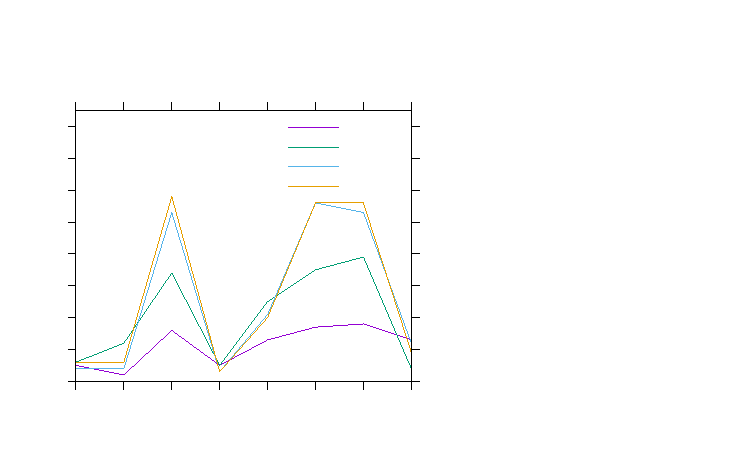
\includegraphics{plot-cairo-2}}%
    \gplfronttext
  \end{picture}%
\endgroup

\caption{Comparison between the number of iterations made by different update parameters when estimating one eigenvalue of a random real symmetric matrix (values from $0$ to $10$), of different size $n$ using the inverse iteration method. The shift is all set to $5$. Furthermore the same matrices are used on all methods for a fair comparison.}
\label{fig2}
\end{figure}

Once again, the number of operations used to find the closest eigenvalue to $5$ seems a bit random, which is an effect of the random matrices in use.
We clearly observe, that all of the methods are attenuated when they reach the number of iterations in which they to the update of the QR-decomposition. This provides evidence that the efficiency of the inverse iteration method can be optimized by introducing a certain update parameter. This advancement of the implementation can as shown be crucial when optimizing the algorithm. However the ideal update parameter might vary from problem to problem, since it for very large problems might be too costly to do the QR-decomposition more than a single time. For a small system it might also be valuable just to do a Jacobi diagonalisation and find all of the eigenvalues, since this procedure is also rather fast. At last we want to compare the method of inverse iteration against one of these Jacobi methods in order to see whether the method is at all relevant, compared to other methods.

\subsection{\label{sec:8}Comparison with Jacobi Method}

At last we want to see whether the inverse iteration algorithm will be able to produce an eigenvalue faster than the previously implemented Jacobi method. This is done through a test where one of each algorithm is timed on the same random matrix with increasing order. Results of this test are shown in Fig. \ref{fig3}.

\begin{figure}[h]
% GNUPLOT: LaTeX picture with Postscript
\begingroup
  \makeatletter
  \providecommand\color[2][]{%
    \GenericError{(gnuplot) \space\space\space\@spaces}{%
      Package color not loaded in conjunction with
      terminal option `colourtext'%
    }{See the gnuplot documentation for explanation.%
    }{Either use 'blacktext' in gnuplot or load the package
      color.sty in LaTeX.}%
    \renewcommand\color[2][]{}%
  }%
  \providecommand\includegraphics[2][]{%
    \GenericError{(gnuplot) \space\space\space\@spaces}{%
      Package graphicx or graphics not loaded%
    }{See the gnuplot documentation for explanation.%
    }{The gnuplot epslatex terminal needs graphicx.sty or graphics.sty.}%
    \renewcommand\includegraphics[2][]{}%
  }%
  \providecommand\rotatebox[2]{#2}%
  \@ifundefined{ifGPcolor}{%
    \newif\ifGPcolor
    \GPcolortrue
  }{}%
  \@ifundefined{ifGPblacktext}{%
    \newif\ifGPblacktext
    \GPblacktexttrue
  }{}%
  % define a \g@addto@macro without @ in the name:
  \let\gplgaddtomacro\g@addto@macro
  % define empty templates for all commands taking text:
  \gdef\gplbacktext{}%
  \gdef\gplfronttext{}%
  \makeatother
  \ifGPblacktext
    % no textcolor at all
    \def\colorrgb#1{}%
    \def\colorgray#1{}%
  \else
    % gray or color?
    \ifGPcolor
      \def\colorrgb#1{\color[rgb]{#1}}%
      \def\colorgray#1{\color[gray]{#1}}%
      \expandafter\def\csname LTw\endcsname{\color{white}}%
      \expandafter\def\csname LTb\endcsname{\color{black}}%
      \expandafter\def\csname LTa\endcsname{\color{black}}%
      \expandafter\def\csname LT0\endcsname{\color[rgb]{1,0,0}}%
      \expandafter\def\csname LT1\endcsname{\color[rgb]{0,1,0}}%
      \expandafter\def\csname LT2\endcsname{\color[rgb]{0,0,1}}%
      \expandafter\def\csname LT3\endcsname{\color[rgb]{1,0,1}}%
      \expandafter\def\csname LT4\endcsname{\color[rgb]{0,1,1}}%
      \expandafter\def\csname LT5\endcsname{\color[rgb]{1,1,0}}%
      \expandafter\def\csname LT6\endcsname{\color[rgb]{0,0,0}}%
      \expandafter\def\csname LT7\endcsname{\color[rgb]{1,0.3,0}}%
      \expandafter\def\csname LT8\endcsname{\color[rgb]{0.5,0.5,0.5}}%
    \else
      % gray
      \def\colorrgb#1{\color{black}}%
      \def\colorgray#1{\color[gray]{#1}}%
      \expandafter\def\csname LTw\endcsname{\color{white}}%
      \expandafter\def\csname LTb\endcsname{\color{black}}%
      \expandafter\def\csname LTa\endcsname{\color{black}}%
      \expandafter\def\csname LT0\endcsname{\color{black}}%
      \expandafter\def\csname LT1\endcsname{\color{black}}%
      \expandafter\def\csname LT2\endcsname{\color{black}}%
      \expandafter\def\csname LT3\endcsname{\color{black}}%
      \expandafter\def\csname LT4\endcsname{\color{black}}%
      \expandafter\def\csname LT5\endcsname{\color{black}}%
      \expandafter\def\csname LT6\endcsname{\color{black}}%
      \expandafter\def\csname LT7\endcsname{\color{black}}%
      \expandafter\def\csname LT8\endcsname{\color{black}}%
    \fi
  \fi
    \setlength{\unitlength}{0.0500bp}%
    \ifx\gptboxheight\undefined%
      \newlength{\gptboxheight}%
      \newlength{\gptboxwidth}%
      \newsavebox{\gptboxtext}%
    \fi%
    \setlength{\fboxrule}{0.5pt}%
    \setlength{\fboxsep}{1pt}%
\begin{picture}(4320.00,2592.00)%
    \gplgaddtomacro\gplbacktext{%
      \csname LTb\endcsname%%
      \put(645,669){\makebox(0,0)[r]{\strut{}$0$}}%
      \csname LTb\endcsname%%
      \put(645,862){\makebox(0,0)[r]{\strut{}$0.5$}}%
      \csname LTb\endcsname%%
      \put(645,1055){\makebox(0,0)[r]{\strut{}$1$}}%
      \csname LTb\endcsname%%
      \put(645,1248){\makebox(0,0)[r]{\strut{}$1.5$}}%
      \csname LTb\endcsname%%
      \put(645,1441){\makebox(0,0)[r]{\strut{}$2$}}%
      \csname LTb\endcsname%%
      \put(645,1633){\makebox(0,0)[r]{\strut{}$2.5$}}%
      \csname LTb\endcsname%%
      \put(645,1826){\makebox(0,0)[r]{\strut{}$3$}}%
      \csname LTb\endcsname%%
      \put(645,2019){\makebox(0,0)[r]{\strut{}$3.5$}}%
      \csname LTb\endcsname%%
      \put(645,2212){\makebox(0,0)[r]{\strut{}$4$}}%
      \csname LTb\endcsname%%
      \put(645,2405){\makebox(0,0)[r]{\strut{}$4.5$}}%
      \csname LTb\endcsname%%
      \put(821,409){\makebox(0,0){\strut{}$100$}}%
      \csname LTb\endcsname%%
      \put(1266,409){\makebox(0,0){\strut{}$200$}}%
      \csname LTb\endcsname%%
      \put(1712,409){\makebox(0,0){\strut{}$300$}}%
      \csname LTb\endcsname%%
      \put(2157,409){\makebox(0,0){\strut{}$400$}}%
      \csname LTb\endcsname%%
      \put(2603,409){\makebox(0,0){\strut{}$500$}}%
      \csname LTb\endcsname%%
      \put(3048,409){\makebox(0,0){\strut{}$600$}}%
      \csname LTb\endcsname%%
      \put(3494,409){\makebox(0,0){\strut{}$700$}}%
      \csname LTb\endcsname%%
      \put(3939,409){\makebox(0,0){\strut{}$800$}}%
    }%
    \gplgaddtomacro\gplfronttext{%
      \csname LTb\endcsname%%
      \put(153,1537){\rotatebox{-270}{\makebox(0,0){\strut{}y}}}%
      \csname LTb\endcsname%%
      \put(2380,130){\makebox(0,0){\strut{}x}}%
      \csname LTb\endcsname%%
      \put(2657,2238){\makebox(0,0)[r]{\strut{}Inverse Iteration}}%
      \csname LTb\endcsname%%
      \put(2657,2052){\makebox(0,0)[r]{\strut{}Jacobi Diag.}}%
    }%
    \gplbacktext
    \put(0,0){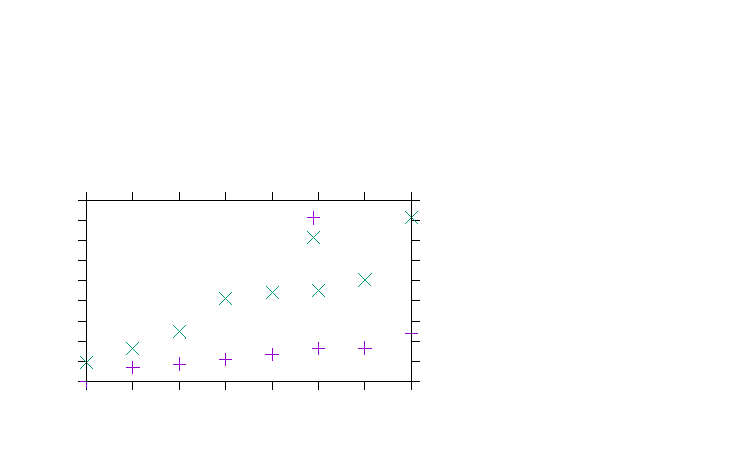
\includegraphics{plot-cairo_time}}%
    \gplfronttext
  \end{picture}%
\endgroup

\caption{Comparison between the computing time by different methods for finding a single eigenvalue of a random real symmetric matrix (values from $0$ to $10$), for different size $n$. Both methods are looking for the lowest eigenvalue on the same matrix.}
\label{fig3}
\end{figure}

The figure clearly show, that the inverse iteration procedure is far superior in computing time as opposed to the Jacobi diagonalization method. The cubed scaling of both methods seem to be the same, but remains lower for the inverse iteration method. This demonstration is even more considerable than at the first look, since the inverse iteration method is even more useful for large systems since it is able to pick out the region in which it will examine opposed to the Jacobi method that will start from the lowest to the highest or opposite. However if one wants to find more than one eigenvalue, then the Jacobi method might be the fastest since it will need less and less iterations the more eigenvalues it determines, as the dimension of the problem in which it solves decreases for each eigenvalue.

\section{\label{sec:9} Conclusion}
A solution of exercise 10 for the final exam has been made. Several methods have been implemented for finding eigenvalues and corresponding eigenvectors with a final refined implementation of an inverse iteration algorithm. To do the calculation a  Golub-Kahan-Lanczos bidiagonalization has been made, thereby also solving exam exercise 9, which will iterate using a calculated matrix-inverse. The refined method however relies on using QR-decomposition by modified Gram-Schmidt orthogonalization to iterate through the solution of a linear system using backsubstitution, based on its advantages for few iterations. An in-depth description and comparison has been made, and an intuitive example has been produced in the out.txt file. For the test, at not point do the algorithms give false results, however a renormalization feature has been implemented to not reach machine-epsilon-related errors. Furthermore all four implementations can be found as functions in the functionfile.c, and the implementation of those concludes the final exam.   


\begin{thebibliography}{9}

\bibitem{GKL}
  Dongarra, J.
  \textit{Golub-Kahan-Lanczos Bidiagonalization Procedure.},
  \href{http://www.netlib.org/utk/people/JackDongarra/etemplates/node198.html}{Netbib.org/...},
  2019.
 
\bibitem{Dmi}
  Fedorov, D.V.
  \textit{Introduction to Numerical Methods},
  Lecture Notes, Aarhus University,
  2019.


\end{thebibliography}

\end{document}


